\documentclass{cta-author}

\newtheorem{theorem}{Theorem}{}
\newtheorem{corollary}{Corollary}{}
\newtheorem{remark}{Remark}{}

\begin{document}

\supertitle{Brief Paper}

\title{Edge matching-based pose tracking for texture-less objects}

\author{\au{Dong Yanchao$^{1}$} \au{Ji Lingling$^2$} \au{Wang Senbo$^3$} \au{Yue Jiguang$^4$} \au{Shen Runjie$^5$} \au{Chen Ce$^5$}}

\address{\add{1}{College of Electronic and Information Engineering, Tongji University, Shanghai, 201804}
\add{2}{Shanghai Institute of Applied Mathematics and Mechanics and Shanghai Key Laboratory of Mechanics in Energy Engineering, Shanghai University, Shanghai, 200072, People's Republic of China}
\email{shanchengcheng2010@163.com}}

\begin{abstract}
\looseness=-1 The paper introduces a novel edge matching-based method for 
estimating and tracking the six degrees of freedom (6DOF) pose for rigid objects
 of arbitrary shapes. In the industrial and augmented reality applications, 
 most targets are texture-less objects. It is difficult to extract feature points 
 from the surface of such objects, which leads to a large error and even failure of the 
 method based on feature points. In the paper, object model and scene gray image are used to 
 construct the loss function by direction chamfer distance tensor, and the tracking problem 
 is transformed into the optimization problem. In order to deal with the situation where the 
 target object is occluded, we propose the adaptive weight optimization algorithm, which uses 
 the direction of the scene image gradient and the edge of the object to judge whether the 
 point is occluded, and calculate the optimal weight by the difference between the two direction.
  Computer Graphics (CG) rendered video, real gray-scale video and public dataset are used to
  evaluate our tracking algorithm. In the Rigid Pose dataset test, the average angle error of 
  our algorithm is $1.835^{\circ}$, 
and the average translation vector error is 0.989 mm, better than the existing methods. 

\end{abstract}

\maketitle

\section{Introduction}\label{sec1}
The Augmented Reality (AR) technology is widely used in various fields both in academic research 
and modern industry [W1]. By flexibly displaying virtual data and image information in real-world 
environments, augmented reality technology can help users review the status of real-world objective 
targets, which suggests that AR systems need reliable methods to estimate the poses of objective targets 
in real-time, particularly methods using only monocular image. In industrial applications, as most objects 
are produced based on fixed precise CAD model, object poses can be retrieved by matching model to object images.
If the input images are from continuous video streams, we also refer the problem as \textbf{“pose tracking system”}.

Most AR targets are texture-rich (which is contradictory to “texture-less”) objects with, 
thus the poses of the objects can be reliably retrieved by feature-point methods [1]. However, 
the poses of texture-less objects (with precise CAD model) cannot be estimated using such manner. 
In industrial applications, many of the objects are made by metal materials and will possibly carry 
texture-less surfaces. Moreover, given that the object pose can be estimated using feature-point-based 
method, it is still difficult to achieve robust and accurate real-time object pose estimation [2, 3].

To be more specific, we believe there are two important challenges we need to overcome when 
formulating a robust and accurate object pose estimation system.
1.  Stably estimate the pose of the object within complex backgrounds. This suggests the system 
should be able to distinguish image projections of 
objects and false positive image features in the backgrounds.
2.	Achieve real-time object pose estimation of texture-less objects. This suggests our 
system should be able to parameterize and describe complex texture-less objects using limited information. 

In this paper, we propose a novel system for object pose estimation for texture-less objects. The proposed 
system iteratively tracks the poses of the object by minimizing the re-projection error of edges 
from object’s CAD model. The reprojection error is estimated by \textbf{Direction Chamfer Matching (DCM) Tensor}.
 Exampled images of the results of the system are shown in Figure 1. 
The main contributions of this paper can be summarized as follows:

1.	Object model and scene gray image are used to construct the loss function by DCM Tensor, 
and the tracking problem is transformed into the optimization problem. Our method replaces the existing 
numerical derivative optimization method with the Jacobian matrix between the 
3D point space coordinates and the coordinates of the corresponding points on the image.
2.	We propose the adaptive weight optimization algorithm, which enables the system to automatically 
reduce the influence of occluded points on the pose optimization, which helps improve tracking accuracy.

\emph{The paper is organized as follows: In Section 2 we review current related works of the 
proposed paper; in Section 3 we detail our pipeline on object pose 
tracking; in Section 4 we test the proposed system and Section 5 concludes this paper.}

\begin{figure}[!h]
  \centering
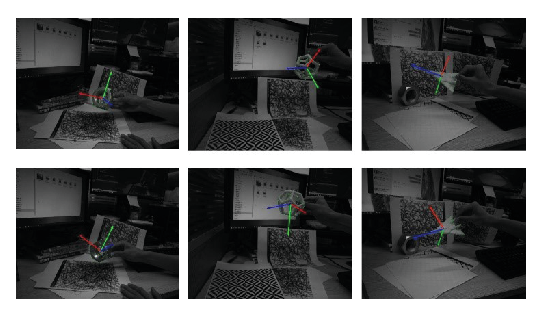
\includegraphics{fig1.eps}
\caption{ Real video tracking. Tracking results of different targets in complex background.}
\label{1}
\end{figure}
  

\section{Related works}\label{sec2}

Many algorithms have been developed to detect and track the target objects. 
Object pose tracking is the basis of unconstrained grabbing techniques for industrial 
components. Initially, the image coordinates of at least four feature points on the surface
 of the object are determined to solve the pose [4, 5, 6]. Estimating object pose using SIFT 
 feature point matching positioning method proposed by Choi \textit{et~al}. in 2008 [7] the translation 
 error of the method is within 5cm and the pose error is within $6^{\circ}$. After that, Youngmin \textit{et~al}. 
 achieved multi-target pose tracking by using feature point extraction and matching 
 methods of key frames [8], improved the efficiency of the tracking algorithm. In 2014, 
 Karl \textit{et~al}. used SIFT feature points to detect objects and achieved segmentation, and then 
 matched object model with depth map information extracted by depth camera to realize multi-target 
 detection and pose tracking [9], the algorithm was tested in the robotic arm grabbing and it takes 
 30ms per frame, the translation error is within 3cm, and the pose error is within $4^{\circ}$. So far, 
 the feature point-based tracking method has met certain requirements in real time and accuracy.

 The matching method based on image edge or contour was first proposed in 1995. 
 By matching the edge of the model with the edge of the image, the method aligns 
 the object model with the edge image of the scene to solve the position and the pose of 
 the object relative to the camera and achieves pose tracking [10] . In 2015, Wang \textit{et~al}. 
 studied the global optimization method of edge matching [11], using the graph model for global 
 optimization. This method also achieved good results in complex background situations.
 The position error is within 2 cm and the pose error is within $4^{\circ}$.

 Spatial point matching method based on random forest[12][13]has ability to track the
  detected object, but the algorithm takes a 
  long time and the error is large. Brachmann \textit{et~al}. [14]using a 
  random forest to classify the pixels of an RGB-D image and estimate 
  the object pose[15]. In recent years, deep learning has also been applied to
   pose estimation. The deep learning based method[16][17]use two-stage approaches, 
   which regress 2D key points firstly and then compute 6D pose parameters, and the 
   result achieve state-of-the-art performance, but when the object is occluded, the system 
   robustness is degraded. Kendall \textit{et~al}.[18] trained CNNs to directly regress the 6D pose of 
   a scene, it has moderate accuracy. The RGB-D pose discrimination algorithm based on deep 
   learning uses the neural network to extract the pose descriptor, and then returns the object 
   position and pose  [19][20][20]. This kind of method still has some disadvantages, such as long 
   time-consuming, 
   high requirements on equipment and unsatisfactory precision.

   The algorithm proposed in this paper mainly solves the problem of pose tracking of
    texture-less objects under complex background [21]. Based on the existing algorithm, 
    the optimization process of the matching between the scene gray image and the object 3D 
    model is improved, and the accuracy and robustness of the registration are improved [22]. 
    The adaptive occlusion weight is constructed by the edge direction of the model and the 
    gradient direction of the scene image, which effectively reduces the influence of mismatched
     points on the overall 
   optimization and improves the accuracy of the tracking algorithm under complex conditions.



\section{Method}\label{sec3}


Compared with the tracking method using detection, the method has higher real-time and continuity,
 and is less prone to error. The pipeline of the algorithm is shown in Figure 2.


\subsection{Method Overview}\label{sec3.1}
In order to achieve the matching between the edge of the object model and the edge of 
the image, one of the commonly used methods is Directional Chamfer Matching (DCM). 
The DCM method [24] improves traditional chamfer matching technology [W2] by using directional matching distance 
along with image coordinate distances. We define DCM error of one group of points $M=\{m_i\}$ using: 

\begin{equation}\label{eq1}
  d_{DCM}(M,N)= {\frac{1}{w}\ \sum_{m_{i}\in \mathcal{M}}\min \limits_{n_{j}\in \mathcal{N}}\\
  (||m_{i}-n_{j}||+\lambda||\phi(m_{i})-\phi(n_{j})||)}
\end{equation}

The $N=\{n_j\}$ is the group of edge points sampled from the image, and the $ n_j $ used in this 
equation represents the edge point with minimal $||m_i-n_J||+\lambda||\phi(m_i)-\phi(n_j)||$ among all edge 
points in N. The $\phi(\cdot)$ represents the edge direction operator in the two-dimensional image.$\lambda$ 
represents the direction error weight. The DCM-based matching method 
can effectively reduce the matching error and is more robust to occlusion and complex background.

The pose of the object can thus be retrieved by matching a group of points from objects onto edges sampled from 
the image. Using $E_"eva"$ to represent DCM of the point group consisted by all points from the object, 
the optimization process can be expressed as: 
\begin{equation}\label{eq2}
  R,T = \arg\min(E_"eva"(T,R))
\end{equation}

The proposed system turns the pose tracking process into continuous estimation of object poses, which 
is an optimization process with adaptive weight. We further detail how we implement the optimization process 
in three parts: loss function definition, weight estimation and details about the optimization process.

\begin{figure}[!h]
\centering
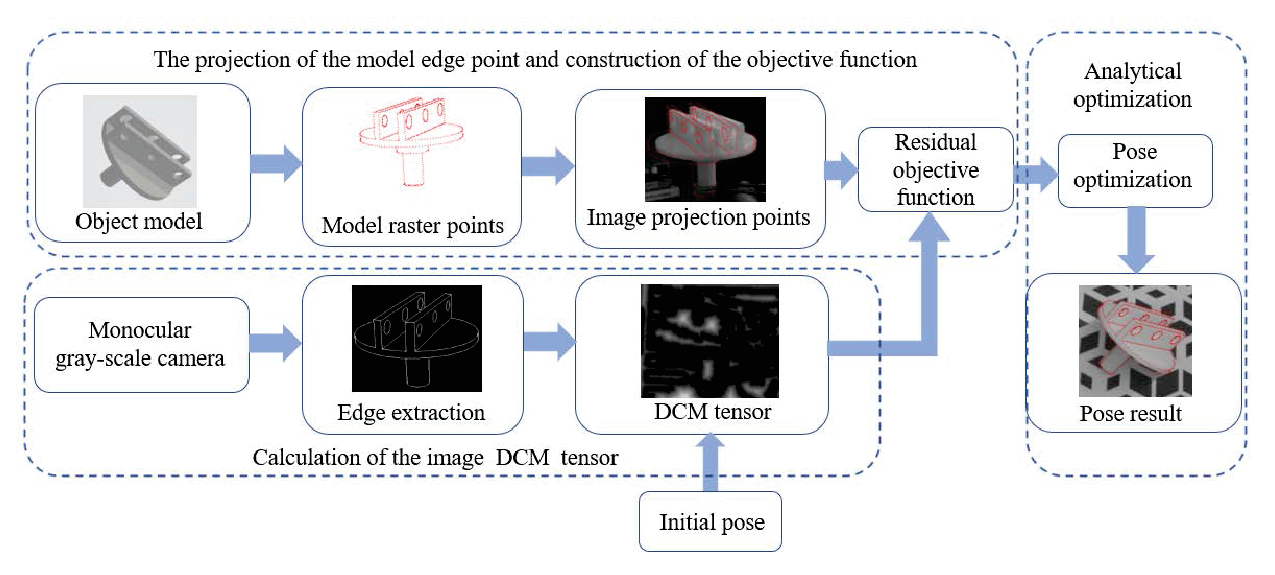
\includegraphics{fig2.eps}
\caption{ Proposed algorithm flowchart.}
\label{2}
\end{figure}

\subsection{Loss Function}\label{sec3.2}
The objective function based on DCM needs to calculate the image coordinates of the 
edge point of the object on the imaging plane of the camera, and the corresponding DCM 
tensor through the edge image, and then obtain the optimized residual corresponding to all
model edge raster points, which is used to obtain the objective function of the overall optimization. 

Firstly, the object depth edge line is extracted by the CAD model of the target object. Secondly, rasterize the edge of the model into a set of three-dimensional discrete point $P={\{o_{1},o_{2},o_{3}...,o_{m}\}}\in \mathbb{R^{3}}$ where the discrete edge points are located on the edge of the object model. The number of discrete edge points directly affects the accuracy of the matching and the efficiency of the algorithm, so we need to weigh these two factors. Through experiments, the raster point spacing is chosen to be 1-2  for the target model in this paper. Get point set $\bar{P}={\{\bar{o}_{1},\bar{o}_{2},\bar{o}_{3},...,\bar{o}_{m}\}}\in \mathbb{R^{3}}$:

\begin{equation}\label{eq3} 
   \bar{o}_i=o_i+\hat{\tau}(o_i)\cdot dr
\end{equation}

Where $\hat{\tau}(o_i)$ represents the edge tangential vector and  represents a small increment, $0<dr\ll 1$.The point set $\bar{p}$ is located in the tangential direction of the edge of the point set $P$ , and the connection direction of the two points represents the corresponding model edge direction. Finally, map raster point sets to image planes using initial poses and camera projection models. Use the initial pose $g\in SE(3)$ to represent the position and pose transformation matrix of the object coordinate system relative to the camera coordinate system in the previous frame or initialization, and map the model edge points to the image coordinate: 

\begin{equation}\label{eq4}
  x_{i}=\pi(o_{i},g)\in \mathbb{R^{2}}, i=\{1,2,3,...,m\}
\end{equation}
\begin{equation}\label{eq5}
\bar{x}_{i}=\pi(\bar{o}_{i},g)\in \mathbb{R^{2}}, i=\{1,2,3,...,m\}
\end{equation}

Where $x_i$ and $\bar{x}_i$  represent the mapping points of $o_i$ and $\bar{o}_i$ in the image plane respectively, and $\pi(\cdot)$ represents the camera projection model.. The next task is to extract the edges of the scene image. In the paper, the LSD algorithm [24] is used to extract the edge of the image. The purpose of the algorithm is to detect the local straight-line contour in the image and form the straight line segment. Compared with other edge extraction algorithms, it can effectively reduce the edge extraction error when the edge length is short, as shown in Figure 3. The LSD edge extraction algorithm is more suitable for the calculation of DCM three-dimensional tensor.


In order to accelerate the direction error calculation of the DCM tensor, in the scene edge image, the edge direction is at an angular interval $\epsilon$ , so that the edges in each angular range are separately formed, as shown in Fig. 4(a). The value of $\epsilon$ affects the edge matching accuracy and the efficiency of the algorithm. Through testing, $\epsilon$ is chosen to be $3^\circ$, namely we divide the edge image into 60 discrete directions. To calculate the DCM tensor, firstly, we calculate the chamfer matching distance for the edge image corresponding to each direction and calculate the distance between all image points and the nearest edge point in the current discrete angle edge. Then the CM tensor of the corresponding discrete angle range edge map is denoted by $DT_V\{\hat{\phi}_i\}$,where $\hat{\phi}_{i},i=\{1,2,3,...,60\}$ represents a discrete edge direction and   represents a current edge image. The calculation result is shown in Fig. 4(b), in which the gray value of the pixel represents the distance of the current pixel from the edge, and the higher the value, the farther the distance. The direction chamfer distance  $DT3_V\{\hat{\phi}_i\}$ is calculated by the chamfer matching distance corresponding to each angle, and the result is shown in Fig. 4(c). The direction chamfer matching tensor is a three-dimensional distance tensor, which represents the minimum edge distance between the image distance and the angular distance of any pixel in different discrete angles. Using the bidirectional dynamic programming algorithm, the direction chamfer distance $DT3_V\{\hat{\phi}_i\}$ of all angles is first initialized to the two-dimensional distance $DT_V\{\hat{\phi}_i\}$ , and the minimum distance corresponding to each point is calculated by forward recursion and backward recursion:

\begin{equation}\label{eq6}
  DT3_{V}(x,\hat{\phi}_{i})=\min\{DT3_{V}(x,\hat{\phi}_{i}),DT3_{V}(x,\hat{\phi}_{i-1})\\
  +\lambda||\hat{\phi}_{i-1}-\hat{\phi}_{i}||_{\pi}\}
\end{equation}
\begin{equation}\label{eq7}
    DT3_{V}(x,\hat{\phi}_{i})=\min\{DT3_{V}(x,\hat{\phi}_{i}),DT3_{V}(x,\hat{\phi}_{i+1})\\
    +\lambda||\hat{\phi}_{i+1}-\hat{\phi}_{i}||_{\pi}\}
\end{equation}

Where $\lambda$ represents the direction error weight. This method is fast in calculation, and can obtain $DT3_{V}(x,\hat{\phi}_{i})$ to all pixel points in each edge image after up to 1.5 forward and backward cycles, and the time complexity is within $\Psi(q)$, where $q$ represents the number of pixels in the image.

After completing the mapping of the model edge raster points and the scene image DCM distance calculation, we construct the direction chamfer matching residual function according to the image coordinates $x_{i}$ of 
the raster points and the direction $\hat{\phi}(x_{i}))$ of the model edge points:

\begin{equation}\label{eq8}
  E_{DCM}={\frac{1}{2}\ \sum_{i=1}^{n}DT3_{V}(x_{i},\hat{\phi}(x_{i}))}
\end{equation}

Where $n$ represents the number of edge points of the object model, and $\hat{\phi}(x_i)$  represents the edge tangential direction of the corresponding edge point in the two-dimensional image, which is the direction in which the point sets $P$ and $\bar{P}$  are mapped to the line after the image coordinate system. Considering the residual function as the objective function we want optimize, we can transform the matching problem into an optimization problem and find the relative pose that makes the sum of the matching residuals of all the raster points minimize. Suppose the relative rotation vector R and the relative translation vector T, the objective function that needs to be optimized can be obtained:

\begin{equation}\label{eq9}
  E(T,R)={\frac{1}{2}\ \sum_{i=1}^{n}DT3_{V}[\pi(o_{i},g(T,R)),\hat{\phi}(\pi(o_{i},g(T,R)))}]^{2}
\end{equation}
Where the $o_{i}$ represents the three-dimensional model edge raster point,$\pi(\cdot)$ represents the 
camera projection model, and $g(T,R)\in \mathbb{R^{6}}$ represents the pose transformation relationship between the object and the camera. By optimizing the objective function $E(T,R)$ to get the accurate pose 
of the target object relative to the camera in the current frame, and  taking the frame pose as the initial pose of the next frame image to achieve pose tracking.


\begin{figure}[!h]
  \centering
  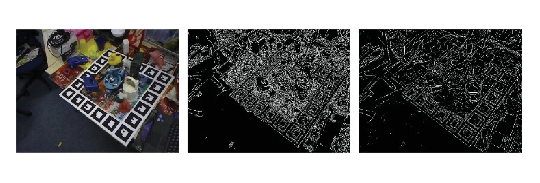
\includegraphics{fig3.eps}
  \caption{ Edge image extracted by different methods. (a) An image of the LINEMOD dataset[25] (b) extracted by Canny algorithms(c) extracted by LSD algorithms}
  \label{3}
  \end{figure}

  \begin{figure}[!h]
    \centering
    
\includegraphics{fig4a.eps}
    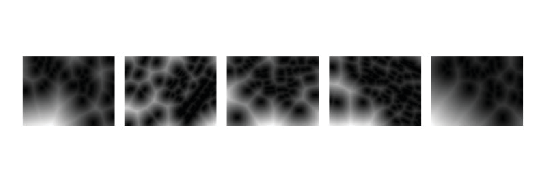
\includegraphics{fig4b.eps}
    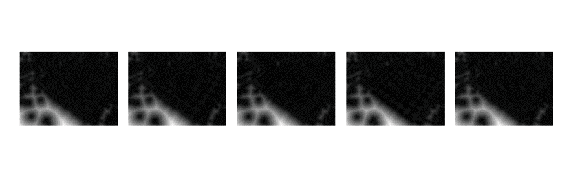
\includegraphics{fig4c.eps}
    \caption{ Computation of the distance transform tensor. (a)  the edge map in different directions. (b)   the two-dimensional distance transform of each direction. (c) the three-dimensional distance transform of each direction.}
    \label{4a}
  \end{figure}




\subsection{Weight Estimation}\label{sec3.3}

In order to improve the robustness of the tracking algorithm under complex background conditions, the paper proposes an algorithm to dynamically change the weight of the raster points to reduce the impact of mismatching points on tracking and improve the accuracy of tracking.

After the matching optimization between the edge image of the current frame and the three-dimensional model of the object is completed, the pose transformation relationship $g(T,R)$ of the object relative to the camera can be obtained. The model edge raster point set $P={\{o_{1},o_{2},o_{3}...,o_{m}\}}\in \mathbb{R^{3}}$ and the adjacent point set$\bar{P}={\{\bar{o}_{1},\bar{o}_{2},\bar{o}_{3},...,\bar{o}_{m}\}}\in \mathbb{R^{3}}$ used to obtain the model edge direction can be mapped to the point set $X=\{x_1,...,x_m\}=\{\pi(o_i,g),i=0,...,m\}\in \mathbb{R^{2}}$and the point set $\bar{X}=\{\bar{x}_1,...,\bar{x}_m\}=\{\pi(\bar{o}_i,g),i=0,...,m\}\in \mathbb{R^{2}}$ in the image plane, respectively. By connecting these two sets of points, the direction of the corresponding model edge $D_{model}(x_i)$ in the image can be calculated. Then extract the gradient direction of the scene image. For image function $f(x,y)$ , its gradient at point $(x,y)$ is a vector with magnitude and direction. Let $G_x$ and $G_y$  represent the gradients in the x  and  y  directions, respectively. The vector of the gradient can be expressed as:


\begin{equation}\label{eq18}
  \nabla f(x,y)=[G_x,G_y ]^T=[\partial f/\partial x,\partial f/\partial y]^T
\end{equation}

The magnitude is:mag $(\nabla f)=\sqrt{((\partial^{2} f)/(\partial x^{2} )+(\partial^{2} f)/(\partial y^{2} ))}$, and the direction is: 
$\phi(x,y)=\arctan \begin{vmatrix} 
  \frac{\partial f}{\partial y} \\
  \frac{\partial f}{\partial x}
  \end{vmatrix}   $. In the paper, the Sobel operator is used to extract the gradient. The operator uses the gradient matrix to convolve with the image matrix, to calculate the gradient approximation of the image gray function, as shown in equation (19, 20), and the error can be effectively reduced.
 
  \begin{equation}\label{eq19}
    G_x= \begin{bmatrix} 
      +1 & 0 & -1\\
      +2 & 0 & -2\\
      +1 & 0 & -1
        \end{bmatrix}*A 
  \end{equation}
  \begin{equation}\label{eq20}
    G_y= \begin{bmatrix} 
      +1 & +2 & +1\\
      0 & 0 & 0\\
      -1 & -2 & -1
        \end{bmatrix}*A 
  \end{equation}

  Where $A$ represents a $3*3$ image matrix centered on the computed point, from which the magnitude $G=\sqrt{{G_x}^2+{G_y}^2}$ and the direction $\Theta=\arctan(G_y/G_x)$ can be obtained.
  
  The magnitude $M_g(x_i)$ and the direction $D_g(x_i)$  of the corresponding point in the image are obtained according to the image coordinate $x_i(u_i,v_i)$  of the model raster point, thereby comparing the model edge direction $D_m(x_i)$  of the point to calculate the optimal weight of the point. First, remove the points with small gradient magnitude. The edges of the images at these points are not obvious. The cause of the problem may be: 
  (1) Due to external reasons such as lighting, the edge of the image is not obvious in the image, and the edge cannot be extracted successfully.
  (2) The edge is occluded. 


  In both cases, the use of the residual of the raster point for pose optimization leads errors. Therefore, the weight of the point to optimize the pose of the next frame should be reduced as much as possible to prevent the influence of mismatched points. Secondly, when the gradient magnitude is larger than the set threshold, it is proved that the matching point has matched the edge of the image, but whether the matching is correct and the accuracy need to be further judged by the model edge direction and the scene image gradient direction. Calculate the weight of the raster point by the following:

\begin{equation}\label{eq21}
  \Xi(x_i)=\begin{cases}
    0.1 , M_g(x_i)<0.01\\
    \sin(D_m(x_i)-D_g(x_i)),M_g(x_i)\geq 0.01
  \end{cases}
\end{equation}

Add optimization weights to the target optimization function:

\begin{equation}\label{eq22}
  E_{eva}(T,R)={\frac{1}{2}\ \sum_{i=1}^{n}\Xi(x_i)\cdot E(T,R)}
\end{equation}
Replace image coordinate point $x_i$  with three-dimensional space point $o_{i}$ :
\begin{equation}\label{eq23}
  E_{eva}(T,R)={\frac{1}{2}\ \sum_{i=1}^{n}\Xi(\pi(o_i,g(T,R))(x_i))\cdot E(T,R)}
\end{equation}
The algorithm we proposed can not only reduce the disturbance caused by the edge extraction error to the system, but also reduce the influence of the interference point on the pose optimization in complex background and improve the robustness of the system.

\subsection{Optimization}\label{sec3.4}

The key to optimize Equation (2) is to find the derivative of A relative to the variable to be optimized. Imperoli [26] optimize the objective function by calculating the numerical derivative. This method performs small perturbation on the optimized variable to calculate an estimation of $\Delta DT3_V$, but it is easy to fall into the local minimum when the initial pose is very “different” with the actual pose. In order to improve the matching accuracy and system robustness, we propose in the paper the analytical method for derivative calculation to improve the robustness and accuracy of the matching. 

The analytical derivative is consisted by two parts: the geometric part and the image part.

Suppose the object coordinate is $C_obj$, the camera coordinate is $C_cam$, T is the relative pose translation between the $C_obj$  and the $C_cam$ ( Lie algebra $\xi$ , rotation matrix R  and the translation vector T), there is a point $p$ on the object coordinate $C_obj$ , which is located at $p^{'}=[x^{'},y^{'},z^{'}]^T$ in $C_cam$ with corresponding point of the camera image as $e=[u,v]$. Given T left by a perturbation 
 $\Delta T=exp(\delta\xi^)$, the operator $\land$ represents the skew-symmetric matrix of vector, and suppose the Lie algebra of the perturbation to $\delta\xi=[\delta\rho,\delta\Phi]^\mathrm{T}$, therefore:
 \begin{equation}\label{eq10}
  \begin{split}
  \frac{\partial (p^{'})}{\partial (\delta\xi)} =\\
  \lim_{\delta\xi\rightarrow 0}\frac{exp(\delta\xi^{\land})exp(\xi^{\land})p-exp(\xi^{\land})p}{\delta\xi}\\
  \approx\lim_{\delta\xi\rightarrow 0}\frac{(I+\delta\xi^{\land})exp(\xi^{\land})p-exp(\xi^{\land})p}{\delta\xi}\\
  =\lim_{\delta\xi\rightarrow 0}\frac{\delta\xi^{\land}exp(\xi^{\land})p}{\delta\xi}\\
  =\lim_{\delta\xi\rightarrow 0}\frac{\begin{pmatrix}
  \partial\phi^{\land}(R_{p}+t) \\
    0
 \end{pmatrix}}{\delta\xi}=\begin{pmatrix}
  I & -(R_{p}+t)^{\land} \\
    0^\mathrm{T} & 0^\mathrm{T}
 \end{pmatrix}
\end{split}
\end{equation}
According to the projection model of the camera:

\begin{equation}\label{eq12}
  \begin{bmatrix} 
    su\\
      sv\\
      s
  \end{bmatrix} 
= \begin{bmatrix} 
        f_{x} & 0 & c_x \\
        0 & f_y & c_y\\
        0& 0 & 1
  \end{bmatrix}
  \begin{bmatrix} 
            x^{'}\\
            y^{'}\\
            z^{'}
  \end{bmatrix} 
\end{equation}

Eliminate the distance of point $p^{'}$ from the camera coordinate:
\begin{equation}\label{eq13}
  \begin{cases}
    u=f_x \frac{x^{'}}{z^{'}}+c_x\\
    v=f_y \frac{y^{'}}{z^{'}}+c_y
  \end{cases}
\end{equation}
Calculate the partial derivative:
\begin{equation}\label{eq14}
\frac{\partial e}{\partial(p^{'})}
=-\begin{bmatrix} 
  \frac{\partial u}{\partial x^{'}} & \frac{\partial u}{\partial y^{'}} & \frac{\partial u}{\partial z^{'}}\\
  \frac{\partial v}{\partial x^{'}} & \frac{\partial v}{\partial y^{'}} & \frac{\partial v}{\partial z^{'}}
\end{bmatrix} 
=-\begin{bmatrix} 
  \frac{f_x}{z^{'}} & 0 & -\frac{f_x x^{'}}{z^{'2}}\\
   0 & \frac{f_y}{z^{'}} & -\frac{f_y y^{'}}{z^{'2}}
\end{bmatrix} 
\end{equation}
According to equations (11) and (14), the Jacobian matrix of the image coordinates of a point on the object relative to the pose transformation can be obtained:
\begin{equation}\label{eq15}
  \frac{\partial e}{\partial \delta\xi}
  =-\begin{bmatrix} 
    \frac{f_x}{z^{'}} & 0 & -\frac{f_x x^{'}}{z^{'2}} & -\frac{f_x x^{'}y^{'}}{z^{'2}} & f_x+\frac{f_x x^{'2}}{z^{'2}} & -\frac{f_x y^{'}}{z^{'}}\\
    0 & \frac{f_y}{z^{'}} &-\frac{f_y y^{'}}{z^{'2}} & -f_y-\frac{f_y y^{'2}}{z^{'2}} & \frac{f_y x^{'}y^{'}}{z^{'2}} & \frac{f_y x^{'}}{z^{'}}
  \end{bmatrix} 
  \end{equation}

  The direction of the model edge point in the image plane is determined by the image coordinates of the raster point and the image coordinates of its neighboring points. Suppose there is a point $p$ on the edge of the model, and there is a neighbouring point $p^{'}$ in the direction of its edge, which is mapped to the camera image plane by the camera projection model, thus getting the point $x(u,v)$ and $\bar{x}(\bar{u},\bar{v})$ respectively,and the connection of the two points is the direction of the edge point in the image plane. It can be obtained:

  \begin{equation}\label{eq17}
    \Phi^{'}=\arctan(\frac{\bar{v}-v}{\bar{u}-u})
    =\frac{1}{1+(\frac{\bar{v}-v}{\bar{u}-u})^{2}}\cdot(\frac{\bar{v}-v}{\bar{u}-u})^{2}
  =\frac{(\bar{v^{'}}-v^{'})(\bar{u}-u)-(\bar{u^{'}}-u^{'}-(\bar{v}-v)}\\
  {(\bar{u}-u)^{2}+(\bar{v}-v)^{'}}
    \end{equation}
    Therefore, the partial derivation of the edge direction relative to the relative pose is:
   \begin{equation}\label{eq18}
    \begin{cases}
     \frac{\partial \Phi}{\partial R}=\frac{(\frac{\partial \bar{v}}{\partial R}-\frac{\partial v}{\partial R})
     (\bar{u}-u)-(\bar{v}-v)(\frac{\partial \bar{u}}{\partial R}-\frac{\partial u}{\partial R})}{(\bar{u}-u)^{2}+(\bar{v}-v)^{2}}\\
     \frac{\partial \Phi}{\partial T}=\frac{(\frac{\partial \bar{v}}{\partial T}-\frac{\partial v}{\partial T})
     (\bar{u}-u)-(\bar{v}-v)(\frac{\partial \bar{u}}{\partial T}-\frac{\partial u}{\partial T})}{(\bar{u}-u)^{2}+(\bar{v}-v)^{2}}

    \end{cases}
      \end{equation}
  Substituting $\partial v/\partial R$ and $\partial U/\partial R$ from Equation (15), the derivatives of the coordinates and directions of the raster points relative to the pose of the object can be obtained. Then, the derivatives of DCM tensors relative to the coordinates and directions of the raster points can be calculated by bilinear interpolation method, and the partial derivatives of DCM tensors relative to the pose change can be obtained.


  \section{Experiments}\label{sec4}
  The algorithm proposed in this paper takes an average of 57ms per frame registration on workstation armed with AMD Ryzen Threadripper 1950x and 32GB RAM. 
  Because of the construction cost of the pose database is too high, and it is difficult to guarantee the accuracy , the paper uses Computer Graphics(CG) technology to render the video to test the accuracy of the algorithm, and uses the rendering software to obtain the true pose of the object relative to the camera. The CG rendered images are shown in Figure 5.
  In this paper, the camera is placed at a different distance from the object to test the tracking accuracy at different scales, as shown in Table 1, where S represents the average size of the object in the image, R represents the average angular deviation, and T represents the average translational deviation.


  TABLE12

  It can be seen from the experimental results that when the average scale of the object is 200~300 pixels, the tracking accuracy is obviously better than the object with the scale of 100 pixels. The main reason is that when the object scale is too small, the number of edge matching points is reduced, the edge extraction accuracy is lowered, and it is more likely to be disturbed.
The test video of the real scene is extracted by a monocular grayscale camera with a resolution of 1280*1024. The accuracy of the algorithm is tested under complex background and lighting conditions. Then use the public database Rigid Pose[28] [29]to test the accuracy of the algorithm, the tracking result is shown in Figure 6. The tracking result is compared with the true value of the database, and the comparison result is shown in Figure 7. The subgraph a-f corresponds to the rotation and translation of the x, y, and z axes in the camera coordinate, where the yellow line represents the true value of the database and the blue line represents the result of the tracking algorithm. The rotation error of our algorithm is $1.835^{\circ}$, and the translation error is 0.989mm. Compared with the sparse point algorithm proposed by Pauwels[30], as shown in Table 2, the advantage of our algorithm is obvious. Compared with the dense tracking method, the translation error of our method is slightly larger, but the algorithm only uses the gray image, which has great advantages in algorithm complexity and computational time. According to the test, the proposed method has good tracking accuracy on CG rendered video, real grayscale video and public dataset. The average rotation error is within $2^{\circ}$ and the average translation error is within 1mm. 
\begin{figure}[!h]
  \centering
  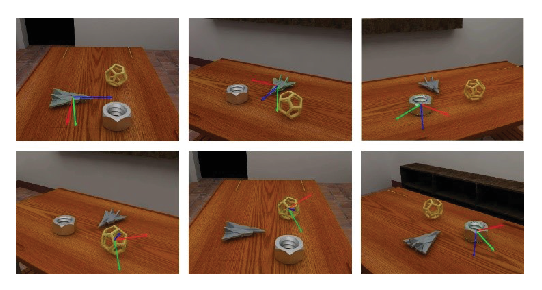
\includegraphics{fig5.eps}
  \caption{ CG rendered video tracking. Use CG rendered video to test the proposed algorithm.}
  \label{5}
  \end{figure}

  \begin{figure}[!h]
    \centering
    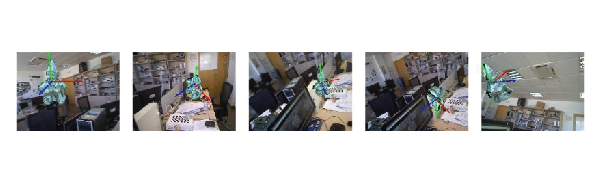
\includegraphics{fig6.eps}
    \caption{Rigid Pose tracking results. Use the public database Rigid Pose to test the proposed algorithm.
      }
    \label{6}
    \end{figure}

  \begin{figure}[!h]
      \centering
      
\includegraphics{fig71.eps}
      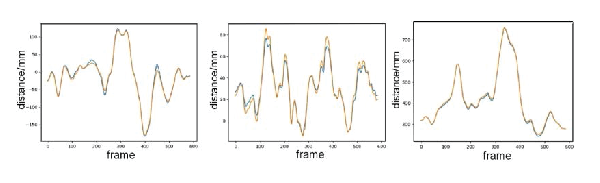
\includegraphics{fig72.eps}
      \caption{Rigid Pose dataset tracking accuracy. The subgraph (a)-(f) respectively corresponds to the rotation and translation of the x, y, and z axes in the camera coordinate, the yellow line represents the true value of the database and the blue line represents the result of the tracking algorithm.}
      \label{7}
  \end{figure}
\section{Conclusions and Future works}\label{sec5}
In this paper, we propose an object tracking algorithm based on the edge of object and construct the direction chamfer residual function, the tracking problem is transformed into the optimization problem by constructing the direction chamfer residual function. The greatest contribution of this paper is to propose an adaptive weight optimization algorithm for the occlusion of the target object, which can not only improve the tracking accuracy in the complex background but also effectively reduces the influence of noise to the tracking. We tested our system with our own rendered untextured objects and the public dataset Rigid Pose in presence of occlusions and cluttered background, the algorithm proved to have high precision and strong robustness. The test shows that the rotation error is within $2^{\circ}$ and the translation error is within 1mm, which has reached the higher level of the existing algorithm. 

In addition, the algorithm saves the computation time and is easy to transplant to the mobile device platform, which makes it have important application value in industrial vision applications. For future works, we want to extend our solution to detect the target objects. This poses new challenges due to the need for simultaneous tracking and detection. Moreover, we intend to further improve the real-time performance of the algorithm.


\section{Acknowledgments}

The work is partially supported by the National Key R\&D Program of China under Grant No.2018YFB1305300, 
the National Natural Science Foundation of China under Grant No. 61873189 and the Natural Science 
Foundation of Shanghai under Grant No. 18ZR1442500.









































\begin{thebibliography}{99}

\bibitem{1}
Vicsek T., Czir\'{o}k A., Ben-Jacob E., Cohen I.: `Novel type of phase transition in a system of self-driven particles', \textit{Phys. Rev. Lett.}, 1995, \textbf{75}, pp.~1226--1229

\bibitem{2}
Jadbabaie A., Lin J., Morse A.S.: `Coordination of groups of
mobile autonomous agents using nearest neighbor rules', \textit{IEEE
Trans. Autom. Control}, 2003, \textbf{48}, pp.~988--1001

\bibitem{3}
Olfati-Saber R., Murray R.M.: `Consensus problems in networks
of agents with switching topology and time-delays', \textit{IEEE Trans.
Autom. Control}, 2004, \textbf{49}, pp.~1520--1533

\bibitem{4}
Ren W., Atkins E.: `Distributed multi-vehicle coordinated
control via local information exchange', \textit{Int. J. Robust
Nonlinear Control}, 2007, \textbf{17}, pp.~1002--1033

\bibitem{5}
Ren W.: `On consensus algorithms for double-integrator dynamics',
\textit{IEEE Trans. Autom. Control}, 2008, \textbf{53}, pp.~1503--1509

\bibitem{6}
Xie G., Wang L.: `Consensus control for a class of networks of
dynamic agents', \textit{Int. J. Robust Nonlinear Control}, 2007,
\textbf{17}, \hbox{pp.~941--959}

\bibitem{7}
Gao Y., Wang L.: `Consensus of multiple dynamic agents with sampled information', \textit{IET Control
Theory Appl.}, 2010, \textbf{4}, pp.~945--956

\bibitem{8}
Tanner H.G., Jadbabaie A., Pappas G.J.: `Flocking in fixed
and switching networks', \textit{IEEE Trans. Autom. Control}, 2007,
\textbf{52}, \hbox{pp.~863--868}

\bibitem{9}
Lee D.J., Spong M.W.: `Stable flocking of multiple inertial
agents on balanced graphs', \textit{IEEE Trans. Autom. Control}, 2007,
\textbf{52}, \hbox{pp.~1469--1475}

\bibitem{10}
Hu J., Lin Y.S.: `Consensus control for multi-agent systems with double-integrator dynamics and time delays', \textit{IET Control
Theory Appl.}, 2010, \textbf{4}, pp.~109--118

\bibitem{11}
Lin P., Jia Y.: `Further results on decentralised coordination
in networks of agents with second-order dynamics', \textit{IET Control
Theory Appl.}, 2009, \textbf{3}, pp.~957--970

\bibitem{12}
Lin P., Jia Y.: `Robust $H_{\infty}$ consensus analysis of a class of second-order multi-agent systems with uncertainty', \textit{IET Control
Theory Appl.}, 2010, \textbf{4}, pp.~487--498

\bibitem{13}
He W., Cao J.: `Consensus control for high-order multi-agent
systems', \textit{IET Control Theory Appl.}, 2011, \textbf{1}, pp.~231--238

\bibitem{14}
Hui Q., Haddad W.M.: `Distributed nonlinear control algorithms
for network consensus', \textit{Automatica}, 2008, \textbf{44}, pp.~2375--2381

\bibitem{15}
Liu X., Chen T., Lu W.: `Consensus problem in directed
networks of multi-agents via nonlinear protocols', \textit{Phys. Lett.
A}, 2009, \textbf{373}, pp.~3122--3127

\bibitem{16}
Zheng Y., Zhu Y., Wang L.: `Consensus of heterogeneous multi-agent systems', \textit{IET Control
Theory Appl.}, 2011, \textbf{5}, pp.~1881--1888

\bibitem{17}
Zhang W., Zeng D., Qu S.: `Dynamic feedback consensus control of a class of high-order multi-agent systems',
\textit{IET Control Theory Appl.}, 2010, \textbf{4}, pp.~2219--2222

\bibitem{18}
Su H.S., Wang X.F., Lin Z.L.: `Flocking of multi-agents with
a virtual leader', \textit{IEEE Trans. Autom. Control}, 2009,
\textbf{54}, pp.~293--307

\bibitem{19}
Song Q., Cao J., Yu W.: `Second-order leader-following
consensus of nonlinear multi-agent system via pinning control', \textit{Syst. Control Lett.}, 2010, \textbf{59}, pp.~553--562

\bibitem{20}
Hong Y.G., Chen G.R., Bushnell L.D.: `Distributed observers
design for leader-following control of multi-agent networks', \textit{Automatica}, 2008, \textbf{44}, pp.~846--850

\bibitem{21}
Hu J., Hong Y.: `Leader-following coordination of multi-agent
systems with coupling time delays', \textit{Physica A}, 2007,
\textbf{374}, pp.~853--863

\bibitem{22}
Ren W.: `Consensus strategies for cooperative control of vehicle
formations', \textit{IET Control Theory Appl.}, 2007, \textbf{1}, pp.~505--512

\bibitem{23}
Khalil H.K.: `Nonlinear systems' (Prentice-Hall, New
Jersey,  2002, 3rd edn.)

\end{thebibliography}

\end{document}
